\chapter{Asking Golf Course Millionaires How They Got Rich}

This episode gives us no blackboard and no formal lecture hall, but it does give us a clear arithmetic of wealth-building. We begin with large sale prices and seven-figure years, then we are forced to solve the problem of access, and only after that do the mechanisms become visible: restrained consumption, diagnostic selling, early investing, capital assembled with leverage rather than outside equity, and scale achieved by repeated operating moves. The right way to read the chapter is therefore the way the episode unfolds itself: first the stakes, then the search, then the machinery.

\section{Preview: Outcomes Before Process}

The lecture opens with a montage of outcomes gathered from later conversations. That is important. We are not yet in the chronology of the day; we are in a preview of what the day will eventually reveal. The opening tells us that the world we are entering contains large exits, seven-digit earning years, and several distinct routes to wealth.

In compressed form, the numerical stakes are these:
\begin{align}
P_{\text{landscape exit}} &\approx \$42\,\text{million},\\
P_{\text{software exit}} &\approx \$38\,\text{million},\\
I_{\text{seven digits}} &\ge \$10^6.
\end{align}

These are not audited financial statements. They are reported markers of scale. Their function in the opening is motivational: they sharpen the question of what sort of decisions, habits, and institutions can plausibly sit behind numbers of this size.

It is already worth noticing that the outcomes are heterogeneous. One number is the sale of a landscape supply company after four years. Another is the sale of a software company. Other numbers refer not to exits but to peak annual income. The lecture does not begin by privileging one ideal path. It begins by telling us that wealth can appear in different commercial forms, and that our task is to look for the common structure underneath.

\section{The Search Structure: Access Before Analysis}

Before the lecture becomes financial, it becomes logistical. The team drives to Austin Country Club, asks if they can do interviews, and is told no unless they are members or residents. This is not dead time. It is the first real obstacle in the lecture, and it matters because it keeps the inquiry honest. Wealth is not simply waiting on an open page; it is gated, and one must first solve the problem of access.

The denial immediately forces a pivot. The game plan changes. A second course is found, the gate is open, and the team gets in, though now with the new problem that attendants are present on every hole. The search structure should stay visible in the notes because it sets the rhythm of everything that follows. The lecture is not built as a single monologue. It is built as a sequence of encounters, each won under conditions of uncertainty.

That is why the opening montage should not be mistaken for the beginning of the actual argument. The actual argument begins here, with the practical problem of reaching the people whose reported outcomes we have just heard.

\section{The First Cluster: Passion, Street Smarts, and the Lagged Lifestyle}

Once inside the second course, the lecture settles into a recurring pattern: ask what someone made, ask what work they did, ask what mechanism mattered, and then ask what advice survives translation into general use. The first interview cluster is about personal formation before it is about corporate structure.

One interviewee reports a peak year a little over a million dollars. When asked about passion, he says it mattered because it allowed him to become a successful hospital administrator doing something he loved and making a difference in people's lives. When asked what led to success, he says: being street smart, always taking the view that there is something to learn each day, and not becoming too full of oneself. The order matters. Passion is not presented as vague self-expression; it is tied to competence, service, and a refusal of arrogance.

Then the lecture turns to financial freedom and becomes more exact. The answer is severe and simple: live within your means. Immediately after that comes the most compact piece of arithmetic in the early part of the episode, a mentor's rule to live on what one made five years ago and invest or bank the rest.

\begin{definition}
Let \(Y_t\) denote income earned in year \(t\), let \(C_t\) denote consumption or lifestyle spending in year \(t\), and let \(S_t\) denote the surplus that can be banked or invested.
\end{definition}

In that notation, the mentor's rule can be written as
\begin{align}
C_t &\approx Y_{t-5},\\
S_t &= Y_t - C_t,\\
Y_t &= C_t + S_t.
\end{align}

\begin{remark}
The relation \(C_t \approx Y_{t-5}\) is not a law of motion derived in the lecture; it is the cleanest formalization of a spoken budgeting rule. Its point is practical rather than theoretical: if consumption is tied to a lagged income level, then current earnings growth is not immediately absorbed by lifestyle inflation.
\end{remark}

This is a real piece of operator arithmetic. The first million, on this telling, is not simply made by increasing gross income. It is made durable by preventing current success from instantly rewriting the standard of living.

The next interviewee shifts the lecture from household arithmetic toward business design. He reports a peak year around \( \$1.5 \) million and says that he is currently a business owner with a golf putting training aid company. When asked what advice he would give someone starting a business this year, the answer is procedural: get advice from people who have successfully launched startups, build a strong business plan, build a strong marketing and social media presence, get funding in place, and take care of your people because they are the ones who will take care of the customer.

So the lecture widens its frame. It moves from personal restraint to the design of a working commercial system.

\section{Intermission and Return}

At this point the lecture interrupts itself with the golf challenge involving James and Will. Analytically, very little is added, but rhythmically the intermission matters. It prevents the first cluster of advice from becoming a flat catalogue. It refreshes the pace and prepares the return to interviews as a second pass through the problem, now with more sharply operational questions.

For that reason the intermission belongs in the chapter, though not at great length. It is not theory, but it is part of the lecture's timing, and the timing affects how the later material lands.

\section{Sales as a Feedback Process}

When the lecture returns, it turns toward sales. One interviewee explains that he was first a golf professional and then moved into IT sales. Asked for his secret to sales, he says that he puts himself in the customer's shoes, tries to build relationships by being personal and real, and listens carefully to what the customer's actual challenges are.

This is already more procedural than inspirational, but the key moment comes one question later, when the host asks how a no becomes a yes.

\subsection{Question \& Answer}

\paragraph{Question.} When a prospect says no, what should we do next?

\paragraph{Answer.} We do not simply push harder. We first ask why the no occurred. The lecture names competition and pricing explicitly, and leaves room for other obstacles. The refusal is treated as information.

In compact form,
\begin{equation}
\text{No} \longrightarrow \{\text{competition},\ \text{pricing},\ \text{other}\}.
\end{equation}

\begin{figure}[h]
\centering
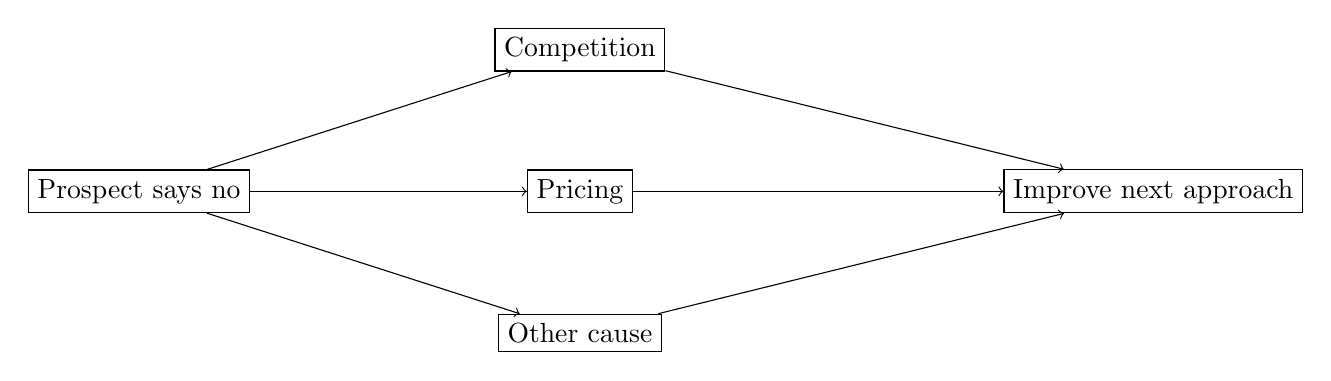
\begin{tikzpicture}[x=2.8cm,y=1.5cm]
\node[draw, rectangle] (no) at (0,0) {Prospect says no};
\node[draw, rectangle] (comp) at (2,1.2) {Competition};
\node[draw, rectangle] (price) at (2,0) {Pricing};
\node[draw, rectangle] (other) at (2,-1.2) {Other cause};
\node[draw, rectangle] (next) at (4.6,0) {Improve next approach};

\draw[->] (no) -- (comp);
\draw[->] (no) -- (price);
\draw[->] (no) -- (other);
\draw[->] (comp) -- (next);
\draw[->] (price) -- (next);
\draw[->] (other) -- (next);
\end{tikzpicture}
\caption{Transcript-derived sales diagnosis. A refusal is not the end of the process; it is classified into a reason and used to sharpen the next attempt.}
\end{figure}

What matters here is the update logic. A failed sale becomes a piece of classified feedback. Sales competence is not merely charm; it is the ability to convert rejection into a more accurate map of the customer's objection.

From there the lecture swings back to personal finance. We hear the blunt warning to stay out of debt, followed by the joke that divorce is expensive because it has already been experienced as such. Then an architect offers a broader comparative claim: many people who did not go to college became financially free because they made good investments, became business owners, and understood that money needed to be invested early.

So this section of the lecture ties together three forms of discipline:
\begin{itemize}
\item relational discipline in sales,
\item behavioral discipline in debt avoidance,
\item temporal discipline in starting investment early.
\end{itemize}

Again the lecture remains empirical. We are not given a formal optimization problem. We are given repeatable mechanisms observed in practice.

\section{Choosing a Game: Employment, Ownership, and Team Alignment}

The next interviews ask a harder question: what kind of commercial game should one actually choose? One speaker says that a college degree is important but not imperative, and that in this country a person can start a business, even using borrowing on the order of a few hundred thousand dollars, if he has a thing he likes to do. He adds the striking anecdote that he himself started a company fifty years ago with \( \$67 \) in the bank.

The lecture then gives that practical claim an ethical condition. The biggest mindset change needed to become a multimillionaire, he says, is humbleness. One should live rightly, refuse conceit, and not imagine that all good fortune was entirely self-caused. This is not neutral managerial language; it belongs to the speaker's own account of how success is to be inhabited.

The same interview then produces a genuine fork in the road. One can choose high-level employment and a very good salary, or one can choose ownership. The point is not that ownership automatically dominates employment. The point is that one must decide who one is, what one is suited for, and what sort of responsibility one is willing to bear.

The software-company interview then carries this problem from the level of career choice to the level of organizational design. The speaker describes a path through Sony and Dell into software, culminating in the sale of PostUp to Upland Software for about \( \$38 \) million. When asked what scaled the company, he answers in the language of placement and coordination: put good people in places where they will be successful, develop them, get everyone on the same page, and make communication effective.

The underlying claim is important. Scale is not presented here as a mystery of valuation. It is presented as a coordination problem. At large companies, he says, politics became a major challenge. In smaller companies, by contrast, one can strip away some of that noise and keep the focus on customer, solution, and product. So the lecture quietly offers us a distinction between two kinds of scale:
\begin{itemize}
\item scale through bureaucracy and accumulated politics,
\item scale through alignment, communication, and focused execution.
\end{itemize}

\section{Capital, Leverage, and the Arithmetic of Growth}

After another brief return to the golf match, the lecture comes back with one of its sharpest bits of financial structure. A later interviewee says that a person should fail a lot, find a mentor quickly, and remember that even a seven-figure year does not solve the main problem. More money means more problems if one does not know how to manage it, keep it, and grow it.

That structure is worth preserving in the shortest possible symbolic form:
\begin{equation}
\text{earn} \longrightarrow \text{keep} \longrightarrow \text{grow}.
\end{equation}

Income is therefore only the first stage. Retention and enlargement of capital are distinct tasks, and failure at those stages can waste a large earnings year.

The same interviewee adds that younger people often lack personal skills, and that those skills matter because much of the available wealth sits above their age bracket. He then offers a very concrete sector claim: medical work is not going away. Here, too, the lecture stays close to lived commercial judgment rather than abstract theory.

The final major case then brings the arithmetic of ownership into its clearest focus. Another speaker says the best advice he would give his younger self is to start his own business. He recounts a path through UT, Wharton, KPMG, PWC, and Union Carbide, then says he became disenchanted with corporate America, bought a landscape supply company in New Braunfels, and sold it four years later for about \( \$42 \) million.

Now the lecture arrives at its strongest practical question.

\subsection{Question \& Answer}

\paragraph{Question.} Do we need investors in order to start or buy a business?

\paragraph{Answer.} The speaker's answer is no, or at least not necessarily. He says there is a great deal of capital available, that investors are often problematic, and that one can use SBA-backed borrowing with a comparatively small cash contribution to reach a viable starting position.

\begin{definition}
Let \(d\) denote the buyer's cash-down fraction:
\begin{equation}
d=\frac{\text{cash down}}{\text{purchase size}}.
\end{equation}
\end{definition}

The lecture gives two explicit examples. If we keep only the arithmetic that is actually spoken, we obtain
\begin{align}
d_{3\text{M}} &= \frac{150{,}000}{3{,}000{,}000} = 0.05 = 5\%,\\
d_{1\text{M}} &= \frac{50{,}000}{1{,}000{,}000} = 0.05 = 5\%.
\end{align}

\paragraph{Worked example.}
\begin{enumerate}
\item We define \(d\) to be the cash-down fraction.
\item For the first example, the lecture gives \( \$150{,}000 \) down on \( \$3{,}000{,}000 \).
\item Therefore
\[
d_{3\text{M}}=\frac{150{,}000}{3{,}000{,}000}=0.05.
\]
\item The second example gives \( \$50{,}000 \) down on \( \$1{,}000{,}000 \).
\item Therefore
\[
d_{1\text{M}}=\frac{50{,}000}{1{,}000{,}000}=0.05.
\]
\item In both spoken examples, the buyer's initial cash is \(5\%\) of the purchase size.
\end{enumerate}

\begin{remark}
These \(5\%\) figures are arithmetic consequences of the examples given in the interview. They are not presented here as universal SBA terms or general lending law.
\end{remark}

This matters because it makes the speaker's claim concrete. The lecture is telling us that entry into ownership may require far less initial equity than the novice imagines, provided the structure of financing can be assembled.

Once that financing question is answered, the lecture closes the loop by returning to the operator's side of scale. The same speaker says that the biggest thing he did was believe in growth. The phrase could easily sound vague, but the details make it precise. Growth means buying more trucks when others doubt that trucks are the right move. Growth means hiring more people when the team is clearly stressed. Growth means buying better equipment. Growth means outsourcing some service function so attention can be kept on the business itself.

So scale is not described as a miracle of branding. It is described as a sequence of bottleneck decisions. When capacity is tight, add capacity. When people are strained, hire. When equipment limits execution, upgrade equipment. When service work absorbs too much managerial attention, push that work outward and reclaim time for the operator's higher-level task.

The lecture's final arithmetic is therefore not only about leverage on the way in. It is also about repeated capacity decisions after entry.

\section{Summary}

The lecture begins by showing us outcomes before it tells us their causes. Then it makes us feel the friction of access. Only after that does it build its case. First we hear the discipline of means: live below current income, let spending lag earnings, and convert growth of income into investable surplus. Then we hear the discipline of sales: a no is not merely a refusal but a reason to be diagnosed. Then we hear the discipline of career choice: know whether you want the game of salaried success or the game of ownership. Finally we hear the arithmetic of ownership itself: investors are not the only path, leverage can lower the entry threshold, and scale is often nothing more glamorous than a series of timely capacity expansions.

That is the mathematical payload of the chapter. It is not formal finance in the textbook sense. It is operator arithmetic: how earnings become surplus, how rejection becomes information, how a small down payment can become control of a larger asset, and how growth becomes a repeated sequence of concrete decisions.